
Para analizar los datos obtenidos del caso de estudio presentado en el capítulo anterior, se visualizó la el caso de estudio de dos formas distintas; la primera una prueba de calidad usando la exactitud y precisión de cada método, y la segunda una prueba de rendimiento donde se comparó los tiempos de cada método.\\

Ya que se busca comparar el método usando AE y AGC para cada modelo, realizamos una comparación entre estos métodos para cada modelo propuesto.\\


\section{Objeto Esférico}

%La comparación del tiempo se realizó con la media de los tiempos. Ya que el método usando AE se realizó con la biblioteca PCL, los tiempos obtenidos con este método son considerados como el punto de comparación, dicho de otra forma, se consideró el tiempo obtenido por el método AE con cada objeto como el cien por ciento del tiempo de ejecución.\\

%En la tabla \ref{tab:tEsf} se muestran los tiempos para la prueba de la \gls{esfera} expresados en porcentajes, donde se observa que usando AGC se obtiene una mejora de tiempo del $13.3\%$ respecto del otro método que usa AE  \\
% 
%
%
%
%\begin{table}
%	\caption{Tiempos para objetos esféricos}
%	\centering
%	\begin{tabular}{lll}
%		\hline
%		&  tiempo(seg.) & tiempo(\%) \\ \hline
%		AE & 2.5284 & 100\% \\
%		AGC & 2.1921 & 86.69\% \\ \hline
%	\end{tabular}
%	\label{tab:tEsf}
%\end{table}

Para comparar la calidad de la clasificación para representar una esfera, se calcula con la ecuación \eqref[ec.]{eq:precision}, ya que los datos se trabajaron en el lenguaje de programación R, para el calculo de la precisión se puede realizar usando el comando $mean()$. \\
%en el caso de la esfera la precisión obtenida se muestra en la tabla \ref{tab:eypesfera},
La precisión calculada para el método usando AE fue de $1.00$, y usando AGC se obtuvo $0.99$, aplicando un criterio en el cual consideramos que si los valores se mantienen en un intervalo de $\pm 0.025$ se consideran como iguales, ya que $-0.025<(1.00-0.99)<0.025$, se obtiene que la precisión entre los métodos no varia. \\

Para la exactitud se evalúa usando la prueba de suma de rangos de Wilcoxon para datos independientes. A continuación se describen los pasos usados en el calculo de la prueba de Wilcoxon para la esfera.\\

En el código \ref{code:cargaDatosEsfera}, para el lenguaje R, se muestra la lectura de los archivos de resultados y se carga en la variable $esferaAE$ y $esferaAGC$, estas son tablas que contienen los tiempos parciales de ejecución, el $veredicto$ es una columna con modelo elegido para representar al objeto, y el $metodo$ se refiere al método usado, $0$para AE, y $1$ para AGC. Se eliminan los casos que no aportan información a la prueba, esto es si no existe un veredicto, lo cual ocurre al inicio cuando aun no se captura la nube de puntos que sera el escenario, así como los que no representaron realizaron una buena representación, para el caso de la esfera el como del $veredicto$ debe contener la palabra $"sphere,"$($"plane,"$para el plano y $"cylinder,"$ para el cilindro), y por ultimo también se quitan los casos cuando se usa un método distinto al deseado.\\


{\small 
	\label{code:cargaDatosEsfera}
	\begin{lstlisting}[caption={Lectura de datos en R.}]
esferaAE <- read.csv("esferaAE.txt",sep="\t")
paraEliminar <- esferaAE\$veredicto == "" | 
	esferaAE$veredicto == ", " | esferaAE$metodo != "0, " |
	esferaAE$veredicto != "sphere, "
esferaAE <- esferaAE[!paraEliminar,]

esferaAGC <- read.csv("esferaAGC.txt", sep="\t")
paraEliminar <- esferaAGC$veredicto == "" | 
	esferaAGC$veredicto == ", " | esferaAGC$metodo != "1, " | 
	esferaAGC$veredicto != "sphere"
esferaAGC <- esferaAGC[!paraEliminar,]
	\end{lstlisting}
}$ $ \\

A continuación en el código \ref{code:rnagosEsfera} se muestra la  seleccionan los primeros treinta datos, de cada método, se juntan los datos en $esferaRank$, y se calcula el rango según el valor obtenido de exactitud, la exactitud fue calculada usando la ecuación \eqref[ec.]{eq:exactitud}.\\


{\small 
	\label{code:rnagosEsfera}
	\begin{lstlisting}[caption={Asignación de rangos.}]
esferaAE30 <- esferaAE[1:30,]
esferaAGC30 <- esferaAGC[1:30,]

esferaRank<-rbind(esferaAE30,esferaAGC30)
esferaRank$rango=rank(esferaRank$exactitud)
	\end{lstlisting}
}$ $ \\

En el código \ref{code:zEsfera}, se observa como se separa el grupo que usa AGC, y se realiza la suma de los rangos y se guarda en la variable $sum$ (el numero $13$ corresponde al indice de la columna de los rangos), se calcula $\mu_r$, $\sigma_R$ y $z$.\\

{\small 
	\label{code:zEsfera}
	\begin{lstlisting}[caption={Calculo de $z$.}]
	paraEliminar <- esferaRank$metodo != "1, "
	esferaRank<-esferaRank[!paraEliminar,]
	sum<-colSums(esferaRank[ ,13, drop=FALSE ])
	
	mu=30*(30+30+1)/2
	sigma=((30*30*(30+30+1))/12)^(1/2)
	###### se calcula z
	Z=(sum-mu)/sigma
	\end{lstlisting}
}$ $ \\

Obteniendo un valor $z=-5.6$, comparando $z$ en el intervalo $[-1.96,1.96]$ se observa que $z<-1.96$ por lo cual la hipótesis nula es descartada, y se afirma que la exactitud obtenida por el método usando AE es diferente a la obtenida por AGC. La media para el método usando AE es $0.9597$ y usando AGC es $0.8581$, con lo cual se asegura que para representar objetos esféricos el método usando AE es mas exacto que usando AGC.




%\begin{table}
%	\caption{Exactitud y precisión de la prueba para la esfera}
%	\centering
%	\begin{tabular}{lll}
%		\hline
%		&  Precisión(\%) & Exactitud(\%) \\ \hline
%		AE & 100\% & 95.97\% \\
%		AGC & 99\% & 85.81\% \\ \hline
%	\end{tabular}
%	\label{tab:eypesfera}
%\end{table}
%
%

 
 


\section{Objeto Plano}

De manera similar a la esfera se calcularon los valores de la exactitud y precisión para un modelo \gls{plano}.\\

Para evaluar la precisión al representar un objeto plano, el valor obtenido usando el método  con AE es de $0.90$ y usando AGC es de $0.94$, aplicando el mismo criterio para el intervalo $\pm 0.025$, se obtiene que $(0.90-0.94)<-0.025$, con lo cual se afirma que la precisión entre los métodos es diferente, y que el método que usa AGC es mas preciso que el que usa AE.\\

Mientras que para la evaluación de la exactitud, se calculo un valor $z=-0.887$, ya que $-1.95<-0.887<1.95$ se confirma la hipótesis nula, la cual afirma que la exactitud de los métodos para representar objetos planos es igual.


%
%En la tabla \ref{tab:tPalno} se muestra el tiempo para el modelo del \gls{plano} expresado en porcentajes, en el cual se observa un incremento del $55.58\%$ de tiempo usando AGC.
%
%
%
%\begin{table}
%	\caption{Tiempos para objetos planos}
%	\centering
%	\begin{tabular}{lll}
%		\hline
%		&  tiempo(seg.) & tiempo(\%) \\ \hline
%		AE & 1.9156 & 100\% \\
%		AGC & 2.9803 & 155.58\% \\ \hline
%	\end{tabular}
%	\label{tab:tPalno}
%\end{table}
%
%De forma similar a la esfera también se comparó la calidad de la clasificación del plano. En la tabla \ref{tab:eypplano} se muestra la precisión y exactitud para ambos métodos. El método usando AGC obtuvo una precisión $4\%$ mayor que aquel con AE. Aplicando la prueba de Wilcoxon se obtuvo un valor $p=0.000464$ el cual denota una diferencia significativa para la exactitud usando AE
%
%\begin{table}
%	\caption{Exactitud y precisión de la prueba para el plano}
%	\centering
%	\begin{tabular}{lll}
%		\hline
%		&  Precisión(\%) & Exactitud(\%) \\ \hline
%		AE & 90\% & 95.97\% \\
%		AGC & 94\% & 85\% \\ \hline
%	\end{tabular}
%	\label{tab:eypplano}
%\end{table}%%%p-value time=1.430546e-18, p-value prob=0.0004646279
%



\section{Objeto Cilíndrico}

Por último tenemos el modelo del \gls{cilindro}. Al igual que para el plano y la esfera se realizaron los cálculos de forma similar.\\

Para evaluar la precisión al representar un objeto cilíndrico, el valor obtenido  usando el método con AE es de $0.47$ y usando AGC es de $0.96$, aplicando el mismo criterio para el intervalo $\pm 0.025$, se obtiene que $(0.47-0.96)<-0.025$, con lo cual se afirma que la precisión entre los métodos es diferente, y que el método que usa AGC es mas preciso que el que usa AE.\\

Mientras que para la evaluación de la exactitud,  se calculo un valor $z=0.761$, ya que $-1.95<0.761<1.95$ se confirma la hipótesis nula, la cual afirma que la exactitud de los métodos para representar objetos cilíndricos es igual.

%
%\begin{table}
%	\caption{Tiempos para objetos cilíndricos}
%	\centering
%	\begin{tabular}{lll}
%		\hline
%		&  tiempo(seg.) & tiempo(\%) \\ \hline
%		AE & 1.7205 & 100\% \\
%		AGC & 1.9997 & 116.23\% \\ \hline
%	\end{tabular}
%	\label{tab:tCyl}
%\end{table}
%
%Por parte de la calidad de la clasificación para el método AGC, en la tabla \ref{tab:eypcilindro} se muestra como la precisión mejora un $49\%$. La prueba de Wilcoxon para comparar la exactitud calcula un valor $p=0.00755$ con el cual se sabe que la exactitud del método usando AGC es mejor que usando AE.
%
%\begin{table}
%	\caption{Exactitud y precisión de la prueba para el cilindro}
%	\centering
%	\begin{tabular}{lll}
%		\hline
%		&  Precisión(\%) & Exactitud(\%) \\ \hline
%		AE & 47\% & 64.17\% \\
%		AGC & 96\% & 71.37\% \\ \hline
%	\end{tabular}
%	\label{tab:eypcilindro}
%\end{table}%%%p-value time=5.777058e-13, p-value prob=0.007557736
%
%En la tabla \ref{tab:ResAna} se muestran las diferencias de los tiempos, precisión y exactitud del método usando AGC y AE.
%
%\begin{table}
%	\caption{Resultados del análisis del caso de estudio}
%	\centering
%	\begin{tabular}{llll}
%		\hline
%		& Tiempo(\%) &  Precisión(\%) & Exactitud(\%) \\ \hline
%		Esfera & -13\% & -1\% & -10.16\% \\
%		Plano & +55.58\% & +4\% & -10.97\% \\
%		Cilindro & +16.23\% & +49\%  & +7.2\%\\ \hline
%		Media & +19.60\% & +17.33\%  & -4.64\%\\
%		 \hline
%	\end{tabular}
%	\label{tab:ResAna}
%\end{table}



\section{Rendimiento}
Para los tiempos de ejecución, en la tabla \ref{tab:tiempos} se muestran los promedios de los tiempos obtenidos para cada etapa del programa descritos anteriormente en la tabla \ref{tab:DefTiempos}. las filas describen el modelo del caso de estudio y el método usado. Para un mejor entendimiento la figura \ref{fig:ttotal} muestra gráficamente los datos obtenidos.\\

\begin{table}[!htb]
	\caption{Resumen de tiempos de la prueba para la esfera usando AE}
	\centering
	\scriptsize 
	\begin{tabular}{llllllllll}
		\hline
		& T1(seg.) & T2(seg.) & T3(seg.) & T4(seg.) & T5(seg.) & T6(seg.) & T7(seg.) & T8(seg.) & T total(seg.) \\ \hline
		Esfera AE & 1.3122 & 0.2956 & 0.3712 & 0.0434 & 0.0088 & 0.2048 & 0.2769 & 0.0142 & 2.5284 \\
		Esfera AGC & 1.0987 & 0.2938 & 0.3985 & 0.0465 & 0.0172 & 0.2184 & 0.0962 & 0.0217 & 2.1921 \\	
		Plano AE & 1.0745 & 0.2671 & 0.3414 & 0.0305 & 0.0128 & 0.0057 & 0.1741 & 0.0093 & 1.9165 \\ 
		Plano AGC & 1.0974 & 0.2716 & 0.3555 & 0.0312 & 0.1715 & 0.0047 & 1.0286 & 0.0190 & 2.9803 \\
		Cilindro AE & 0.8806 & 0.2962 & 0.3821 & 0.0245 & 0.0247 & 0.0137 & 0.0831 & 0.0146 & 1.7205 \\
		Cilindro AGC & 0.9730 & 0.2947 & 0.3775 & 0.0231 & 0.0447 & 0.0135 & 0.2322 & 0.0404 & 1.9997 \\
		
		\hline
	\end{tabular}
	\label{tab:tiempos}
\end{table}


\begin{figure}[!htb]
	\centering
	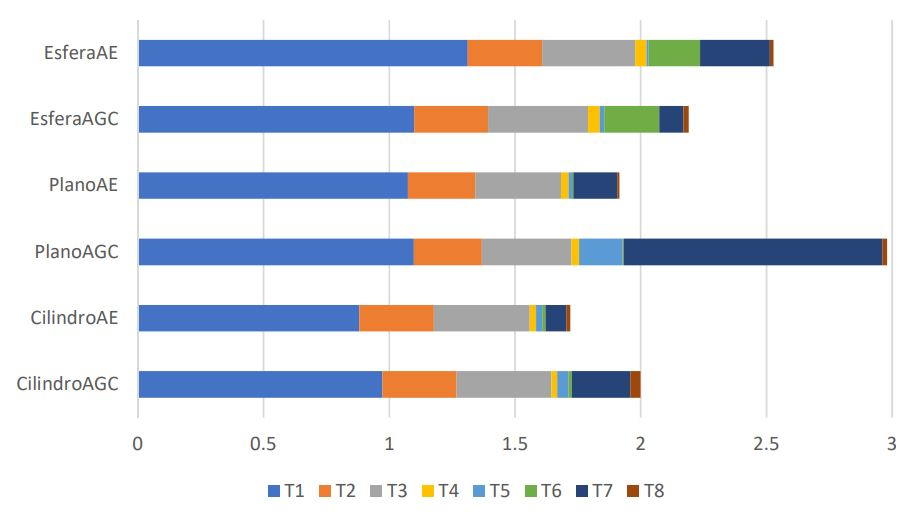
\includegraphics[width=1\textwidth]{03Resultados/imagenes/tTotal.JPG}
	\caption{Tiempos promedios de la prueba} 
	\label{fig:ttotal} 
\end{figure}


